
% -- ----------------------------------------------------------------------------------------- -- #
% -- Initial Developer: IF Francisco ME ------------------------------------------------------ -- #
% -- GitHub Repossitory:  -------------------------------------------------------------------- -- #
% -- License: GNU General Public License ----------------------------------------------------- -- #
% -- ----------------------------------------------------------------------------------------- -- #

\documentclass[final, xcolor=table]{beamer}\usepackage[]{graphicx}\usepackage[]{color}
%% maxwidth is the original width if it is less than linewidth
%% otherwise use linewidth (to make sure the graphics do not exceed the margin)
\makeatletter
\def\maxwidth{ %
  \ifdim\Gin@nat@width>\linewidth
    \linewidth
  \else
    \Gin@nat@width
  \fi
}
\makeatother

\definecolor{fgcolor}{rgb}{0.345, 0.345, 0.345}
\newcommand{\hlnum}[1]{\textcolor[rgb]{0.686,0.059,0.569}{#1}}%
\newcommand{\hlstr}[1]{\textcolor[rgb]{0.192,0.494,0.8}{#1}}%
\newcommand{\hlcom}[1]{\textcolor[rgb]{0.678,0.584,0.686}{\textit{#1}}}%
\newcommand{\hlopt}[1]{\textcolor[rgb]{0,0,0}{#1}}%
\newcommand{\hlstd}[1]{\textcolor[rgb]{0.345,0.345,0.345}{#1}}%
\newcommand{\hlkwa}[1]{\textcolor[rgb]{0.161,0.373,0.58}{\textbf{#1}}}%
\newcommand{\hlkwb}[1]{\textcolor[rgb]{0.69,0.353,0.396}{#1}}%
\newcommand{\hlkwc}[1]{\textcolor[rgb]{0.333,0.667,0.333}{#1}}%
\newcommand{\hlkwd}[1]{\textcolor[rgb]{0.737,0.353,0.396}{\textbf{#1}}}%
\let\hlipl\hlkwb

\usepackage{framed}
\makeatletter
\newenvironment{kframe}{%
 \def\at@end@of@kframe{}%
 \ifinner\ifhmode%
  \def\at@end@of@kframe{\end{minipage}}%
  \begin{minipage}{\columnwidth}%
 \fi\fi%
 \def\FrameCommand##1{\hskip\@totalleftmargin \hskip-\fboxsep
 \colorbox{shadecolor}{##1}\hskip-\fboxsep
     % There is no \\@totalrightmargin, so:
     \hskip-\linewidth \hskip-\@totalleftmargin \hskip\columnwidth}%
 \MakeFramed {\advance\hsize-\width
   \@totalleftmargin\z@ \linewidth\hsize
   \@setminipage}}%
 {\par\unskip\endMakeFramed%
 \at@end@of@kframe}
\makeatother

\definecolor{shadecolor}{rgb}{.97, .97, .97}
\definecolor{messagecolor}{rgb}{0, 0, 0}
\definecolor{warningcolor}{rgb}{1, 0, 1}
\definecolor{errorcolor}{rgb}{1, 0, 0}
\newenvironment{knitrout}{}{} % an empty environment to be redefined in TeX

\usepackage{alltt}
\usepackage[orientation=portrait,size=a0,scale=1.4]{beamerposter}
\usetheme{FichaTecnica}
\usepackage{graphicx}
\usepackage{booktabs}
\usepackage[spanish]{babel}
\usepackage{amsmath,amsthm,amssymb,latexsym}
\usepackage{booktabs}
\usepackage{ragged2e}
\graphicspath{{figures/}}


































% -- -------------------------------------------------------------------------------------------- %
%	-- TITLE SECTION 
% -- -------------------------------------------------------------------------------------------- %

\title{\Huge Econometrics for time series analysis }

% -- -------------------------------------------------------------------------------------------- %
%	-- FOOTER TEXT
% -- -------------------------------------------------------------------------------------------- %

\newcommand{\leftfoot}{Official Web }
\newcommand{\rightfoot}{More Info \textbf{if.francisco.me@gmail.com}}

% -- -------------------------------------------------------------------------------------------- %
\IfFileExists{upquote.sty}{\usepackage{upquote}}{}
\begin{document}

% -- ----------------------------------------------------------------------------------------- -- %
% -- -- Row 1 -- Dialy Prices ---------------------------------------------------------------- -- %
% -- ----------------------------------------------------------------------------------------- -- %

\begin{columns}[t]

% -- ------------------------------------------------------------------------------- Columna 1 -- %
% -- ----------------------------------------------------------------------------------------- -- %

\begin{column}{.66 \linewidth}

  \begin{block}{Price Time Series}

  \begin{figure}[H]
    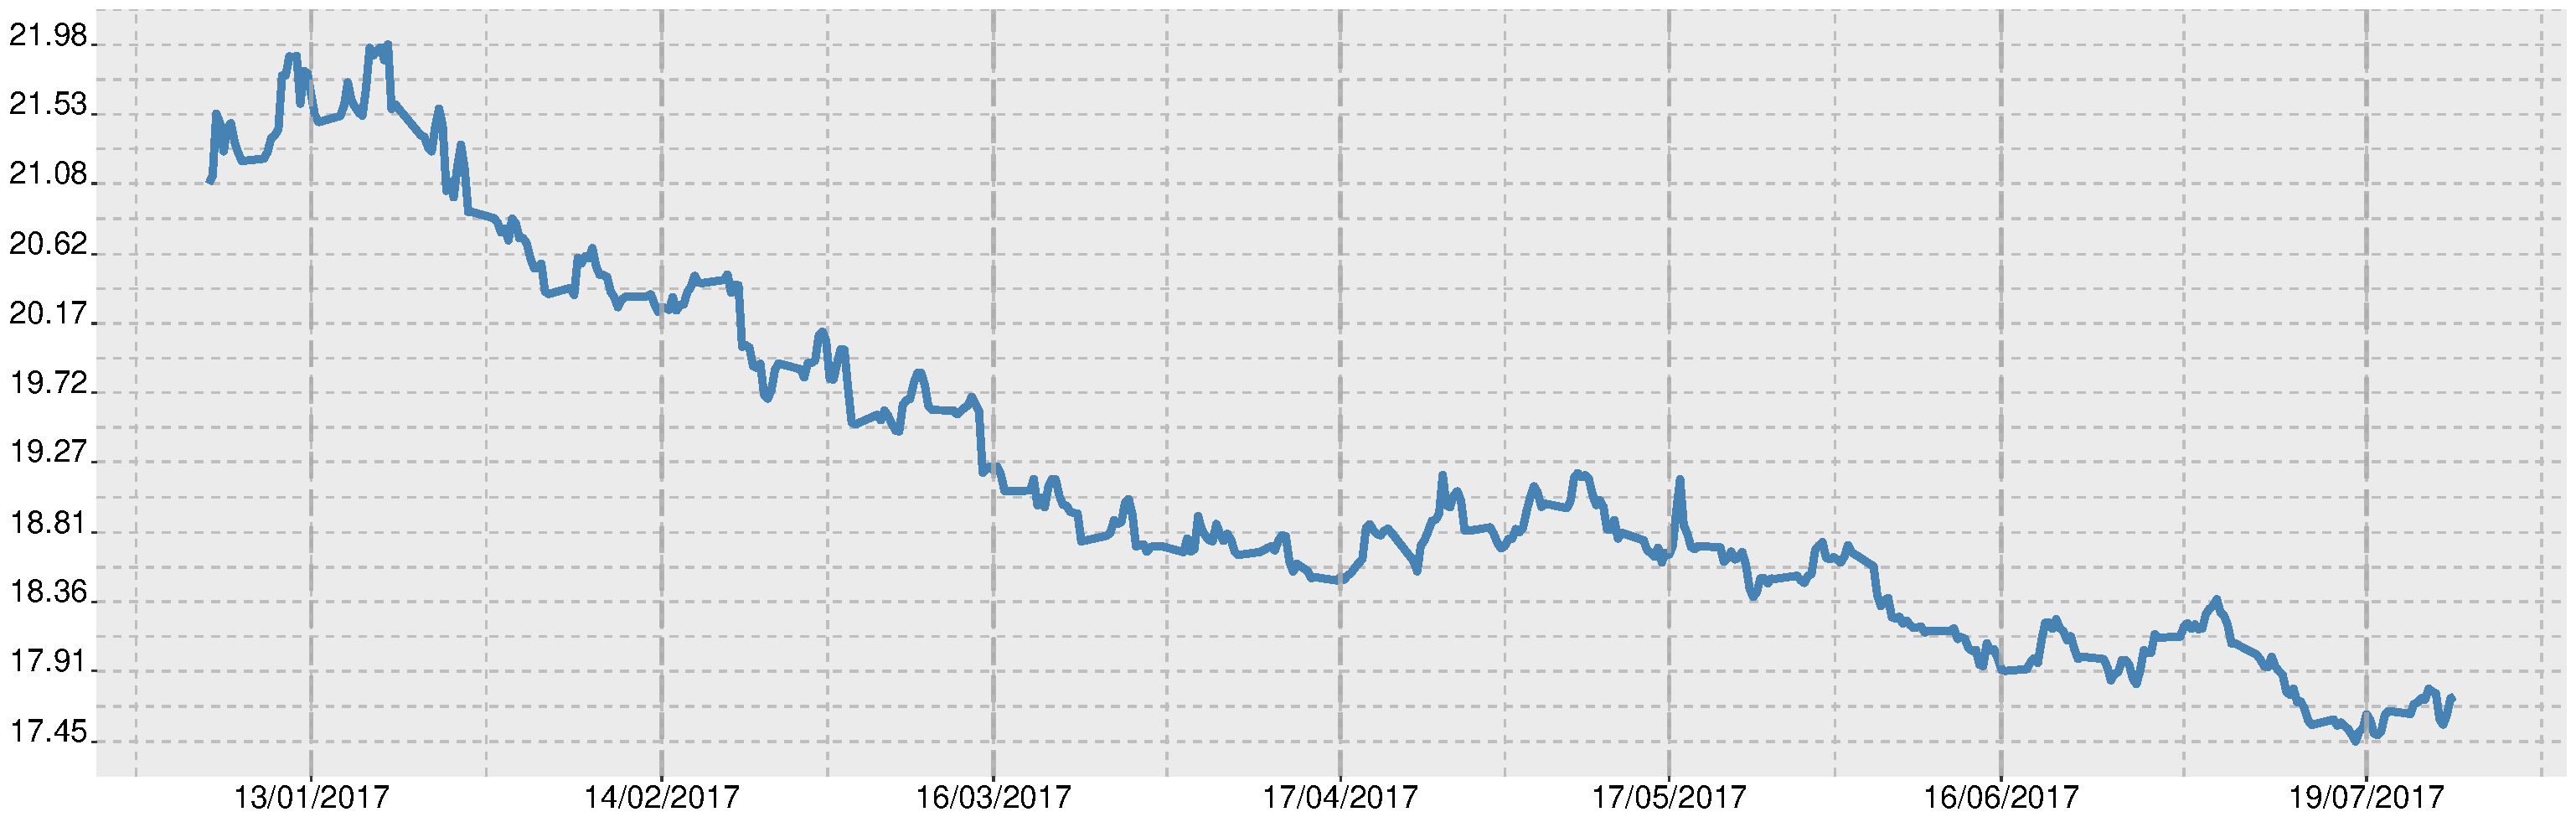
\includegraphics[scale=1]{figure/Plot_ts-1.pdf}
  \end{figure}

  \end{block}
  
\end{column}

% -- ------------------------------------------------------------------------------- Columna 2 -- %
% -- ----------------------------------------------------------------------------------------- -- %

\begin{column}{.32 \linewidth}
  
  \begin{block}{Price Data}
  
  \centering
  
\begin{tabular}{l|l}
\hline
Value & Parameter\\
\hline
Observations & 471\\
\hline
Start Date & 2017-01-03 15:00:00\\
\hline
Min Value & 17.45\\
\hline
Mean & 19\\
\hline
Median & 18.8168\\
\hline
Standar Deviation & 1.17703285640164\\
\hline
Max Value & 21.9842\\
\hline
End Date & 2017-07-27 15:00:00\\
\hline
\end{tabular}


 
 
  \end{block}
  
\end{column}

\end{columns}

% -- ----------------------------------------------------------------------------------------- -- %
% -- -- Row 2 -- 8 Hour Prices --------------------------------------------------------------- -- %
% -- ----------------------------------------------------------------------------------------- -- %

\begin{columns}[t]

% -- ------------------------------------------------------------------------------- Columna 1 -- %
% -- ----------------------------------------------------------------------------------------- -- %

\begin{column}{.32 \linewidth}

  \begin{block}{Statistical Tests}

    \begin{itemize}
    
      \item Serial Auto Correlation: Llung-Box \\
            p.value: 0 \\
      
      \item Normality: Kolgomorov-Smirnoff \\
            p.value: 0 \\
            
      \item Heteroscedascity:  McLeod-Li\\
            p.value: 0 \\
    
    \end{itemize}
  

  \end{block}
  
\end{column}

% -- ------------------------------------------------------------------------------- Columna 2 -- %
% -- ----------------------------------------------------------------------------------------- -- %

\begin{column}{.32 \linewidth}

  \begin{block}{Serial (Cumulative) Auto Correlation}

   \begin{figure}[H]
    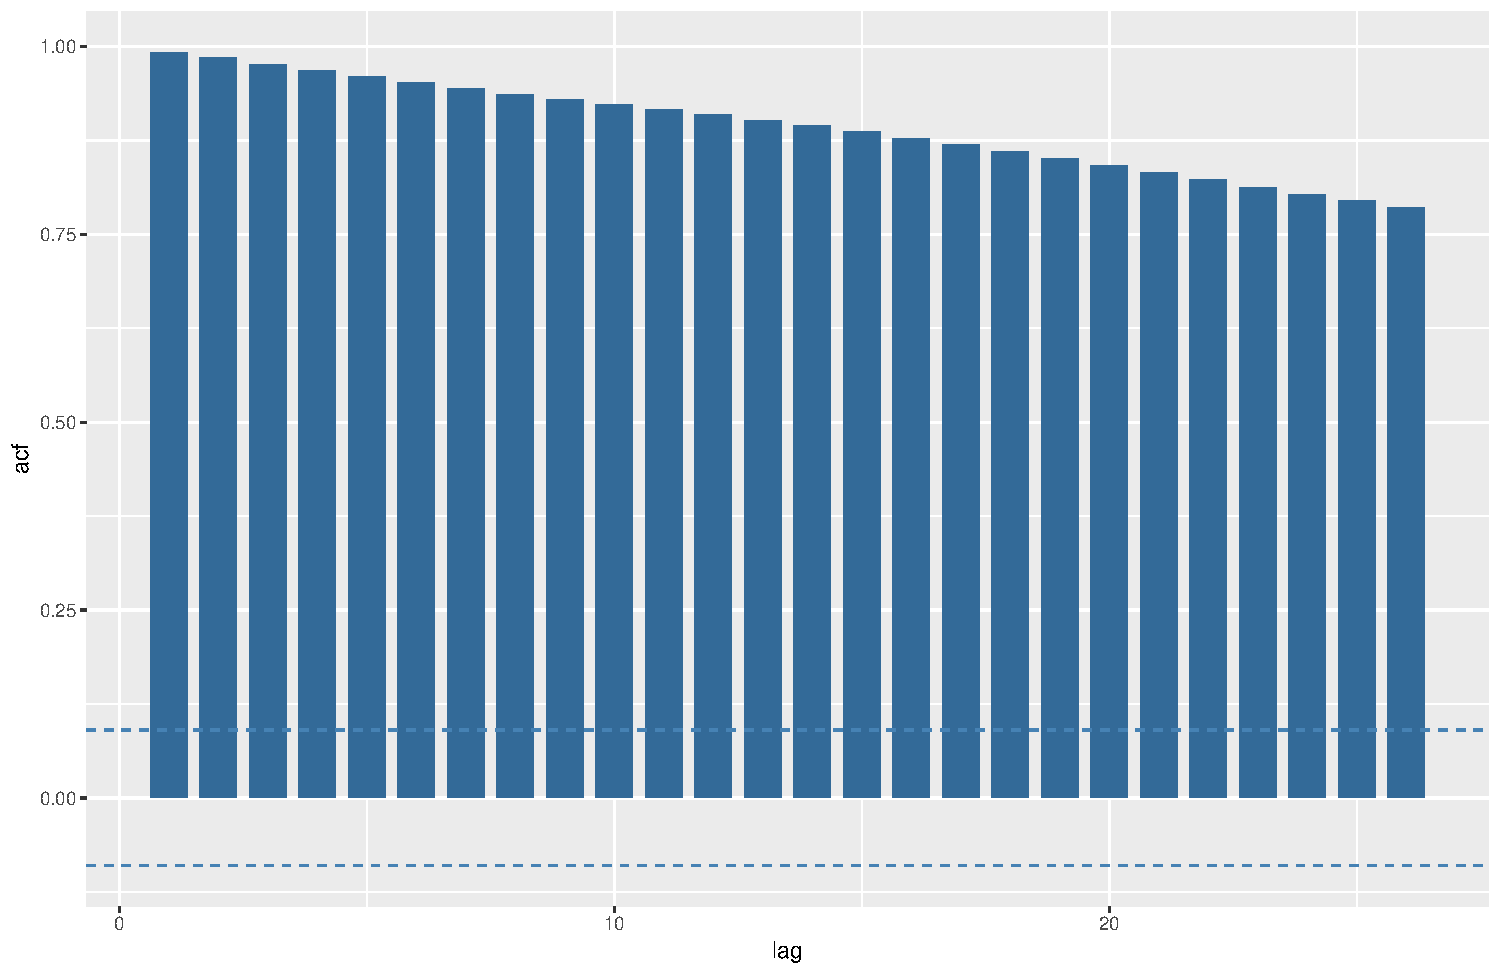
\includegraphics[scale=1]{figure/Plot_acf-1.pdf}
    \end{figure}

  \end{block}
  
\end{column}

% -- ------------------------------------------------------------------------------- Columna 3 -- %
% -- ----------------------------------------------------------------------------------------- -- %

\begin{column}{.32 \linewidth}

  \begin{block}{Partial Auto Correlation}

   \begin{figure}[H]
    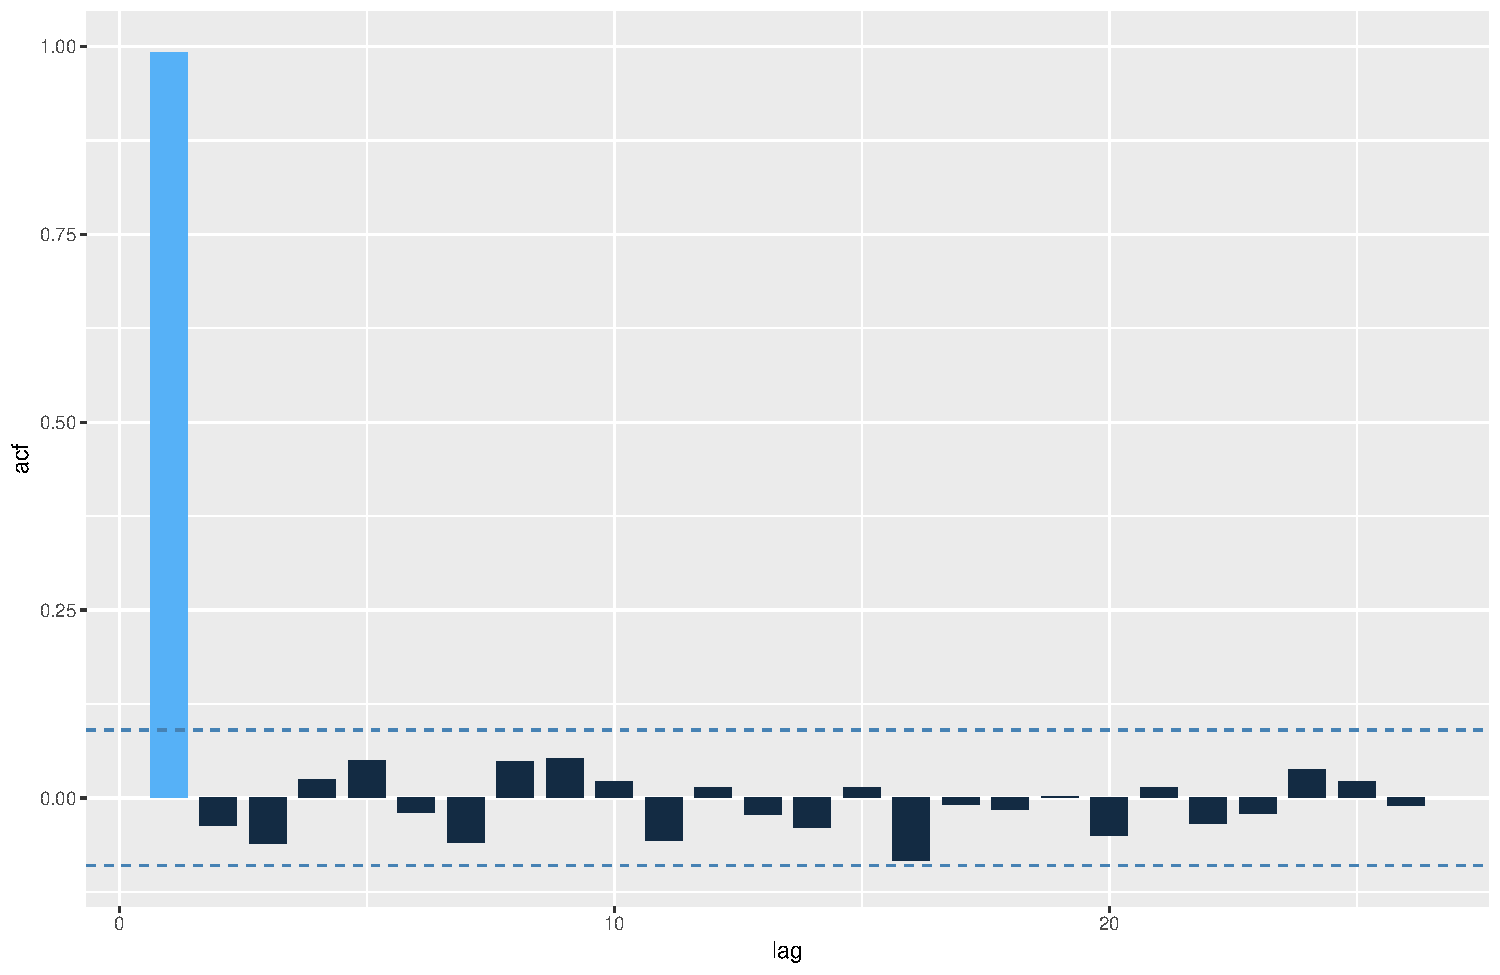
\includegraphics[scale=1]{figure/Plot_acf-2.pdf}
    \end{figure}

  \end{block}
  
\end{column}
\end{columns}

% -- ----------------------------------------------------------------------------------------- -- %
% -- -- Row 3 -- 8 Hour Prices --------------------------------------------------------------- -- %
% -- ----------------------------------------------------------------------------------------- -- %

\begin{columns}[t]

% -- ------------------------------------------------------------------------------- Columna 1 -- %
% -- ----------------------------------------------------------------------------------------- -- %

\begin{column}{.66 \linewidth}

  \begin{block}{Price Time Series}

  \begin{figure}[H]
    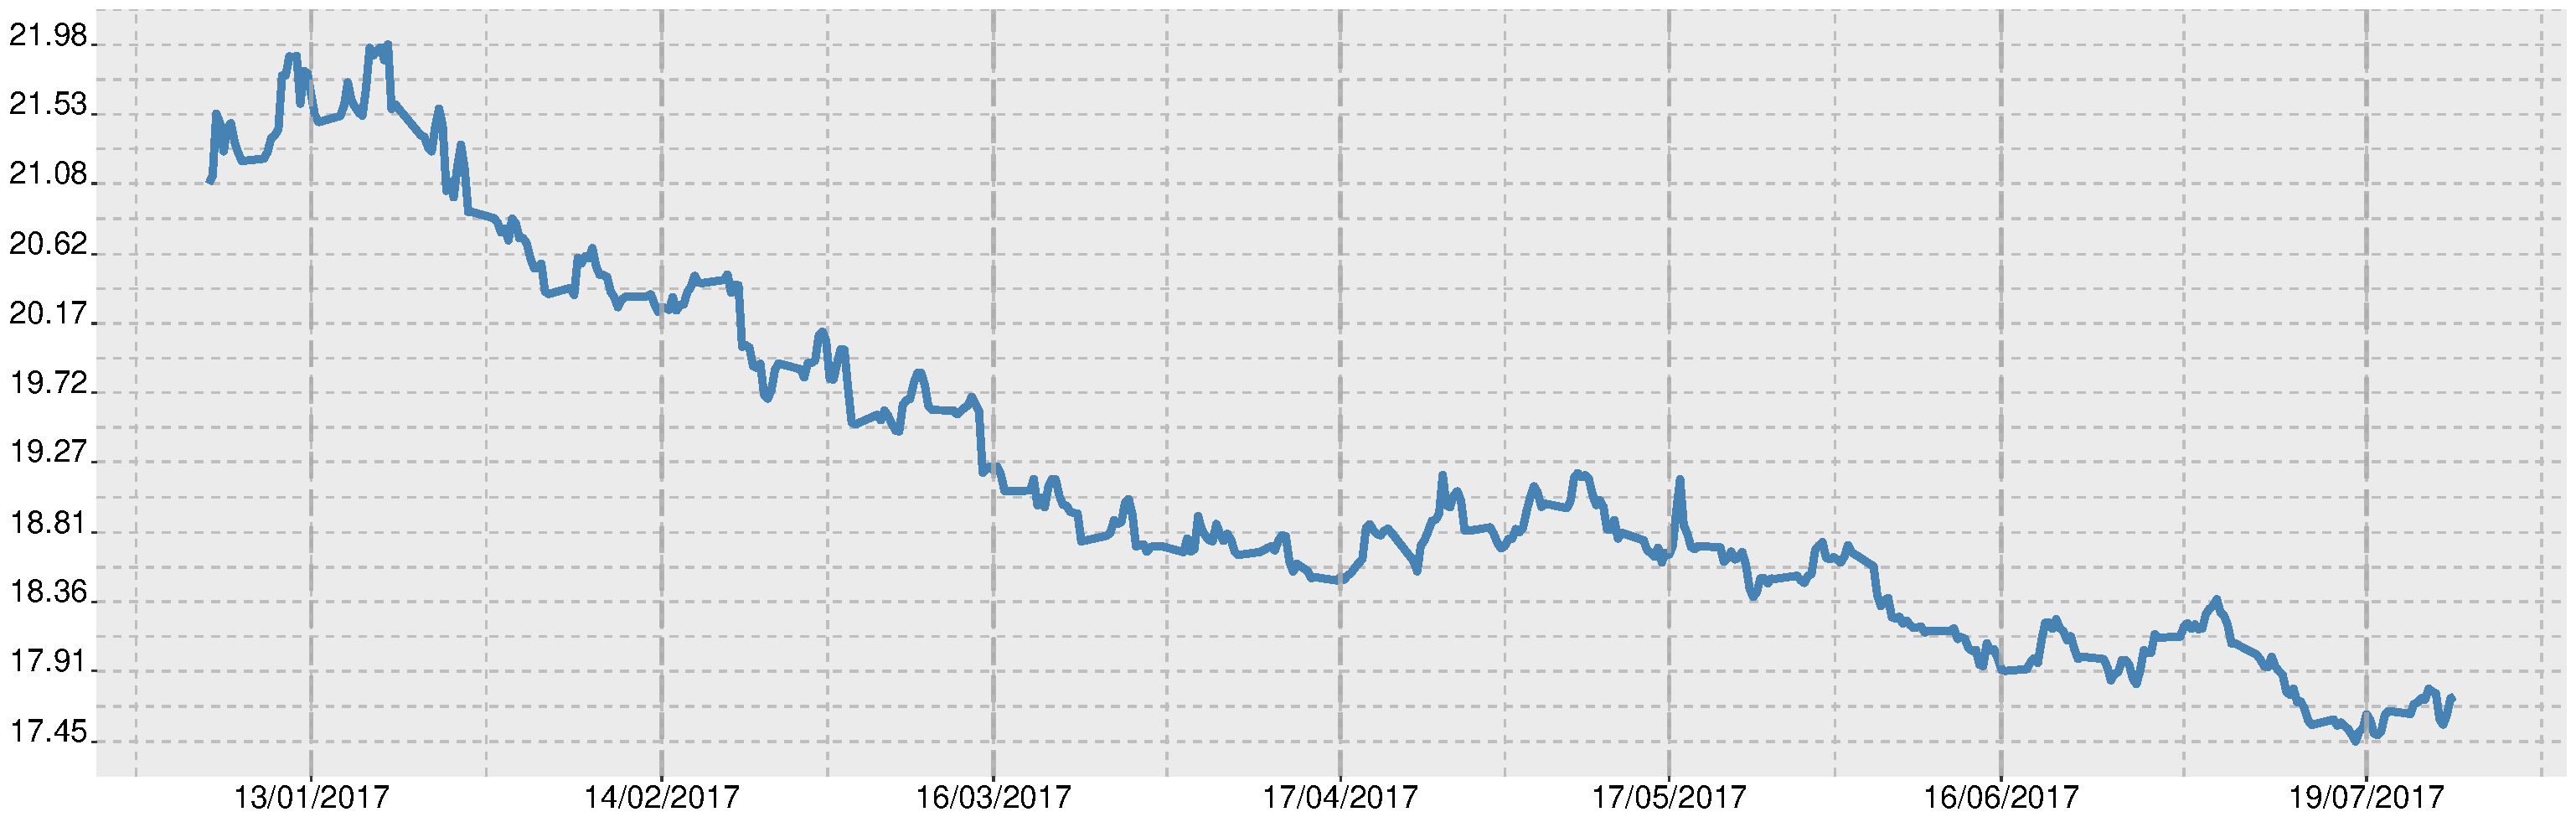
\includegraphics[scale=1]{figure/Plot_ts-1.pdf}
  \end{figure}

  \end{block}
  
\end{column}

% -- ------------------------------------------------------------------------------- Columna 2 -- %
% -- ----------------------------------------------------------------------------------------- -- %

\begin{column}{.32 \linewidth}
  
  \begin{block}{Price Data}
  
  \centering
  
\begin{tabular}{l|l}
\hline
Value & Parameter\\
\hline
Observations & 471\\
\hline
Start Date & 2017-01-03 15:00:00\\
\hline
Min Value & 17.45\\
\hline
Mean & 19\\
\hline
Median & 18.8168\\
\hline
Standar Deviation & 1.17703285640164\\
\hline
Max Value & 21.9842\\
\hline
End Date & 2017-07-27 15:00:00\\
\hline
\end{tabular}


 
 
  \end{block}
  
\end{column}

\end{columns}

% -- ----------------------------------------------------------------------------------------- -- %
% -- -- Row 4 -- 8 Hour Prices --------------------------------------------------------------- -- %
% -- ----------------------------------------------------------------------------------------- -- %


\begin{columns}[t]

% -- ------------------------------------------------------------------------------- Columna 1 -- %
% -- ----------------------------------------------------------------------------------------- -- %

\begin{column}{.49 \linewidth}

  \begin{block}{Close - Open}

    \begin{figure}[H]
      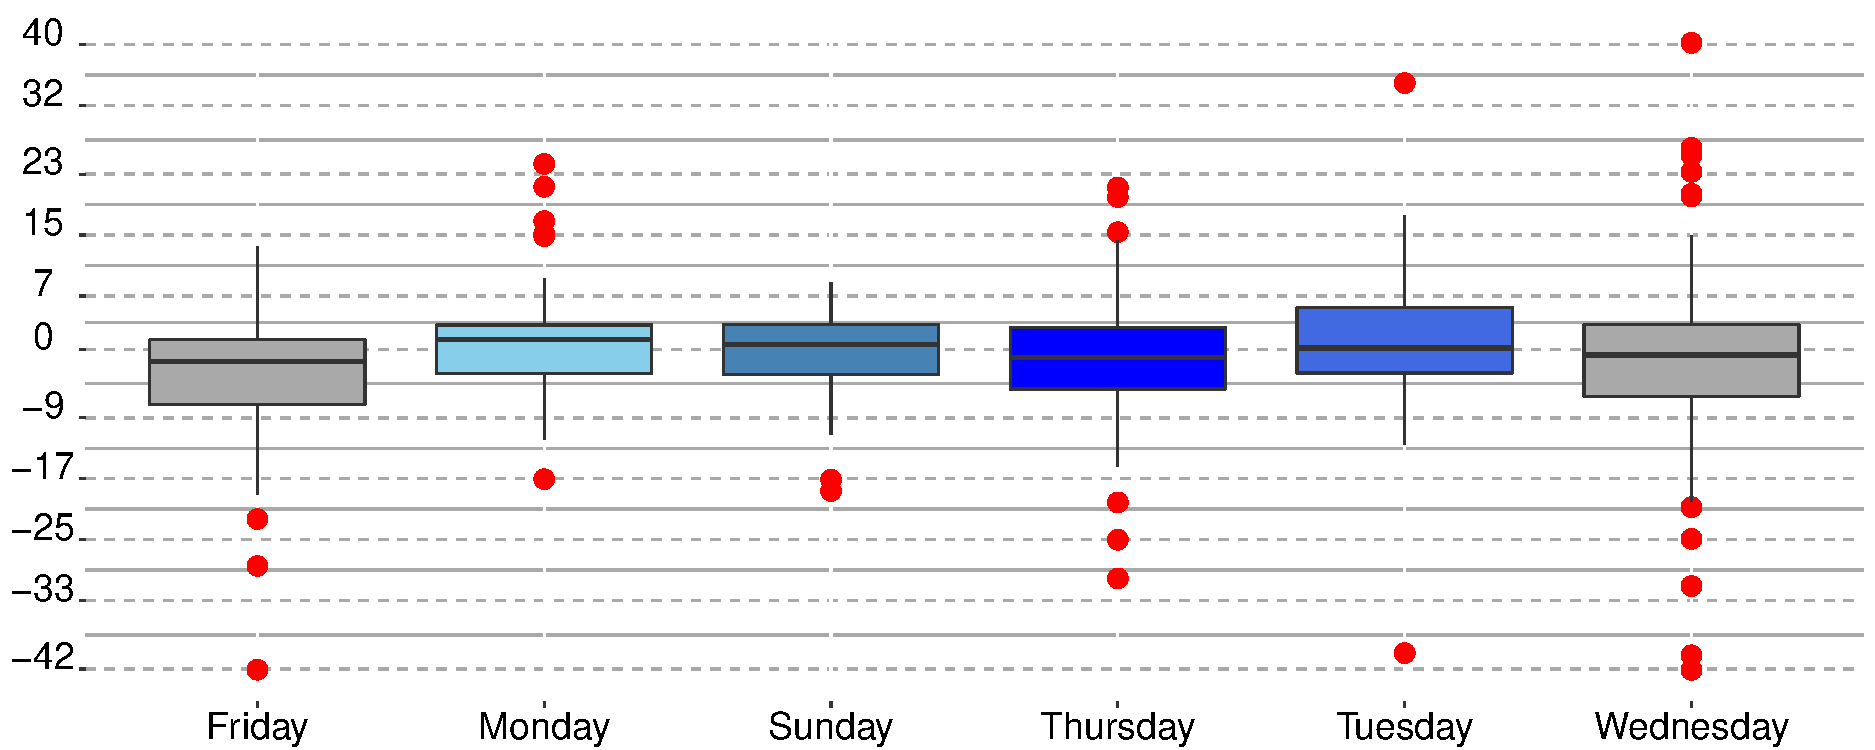
\includegraphics[scale=1]{figure/BP_Plot-1.pdf}
    \end{figure}
    
  \end{block}
  
\end{column}

% -- ------------------------------------------------------------------------------- Columna 2 -- %
% -- ----------------------------------------------------------------------------------------- -- %

\begin{column}{.49 \linewidth}

  \begin{block}{High - Low}

   \begin{figure}[H]
    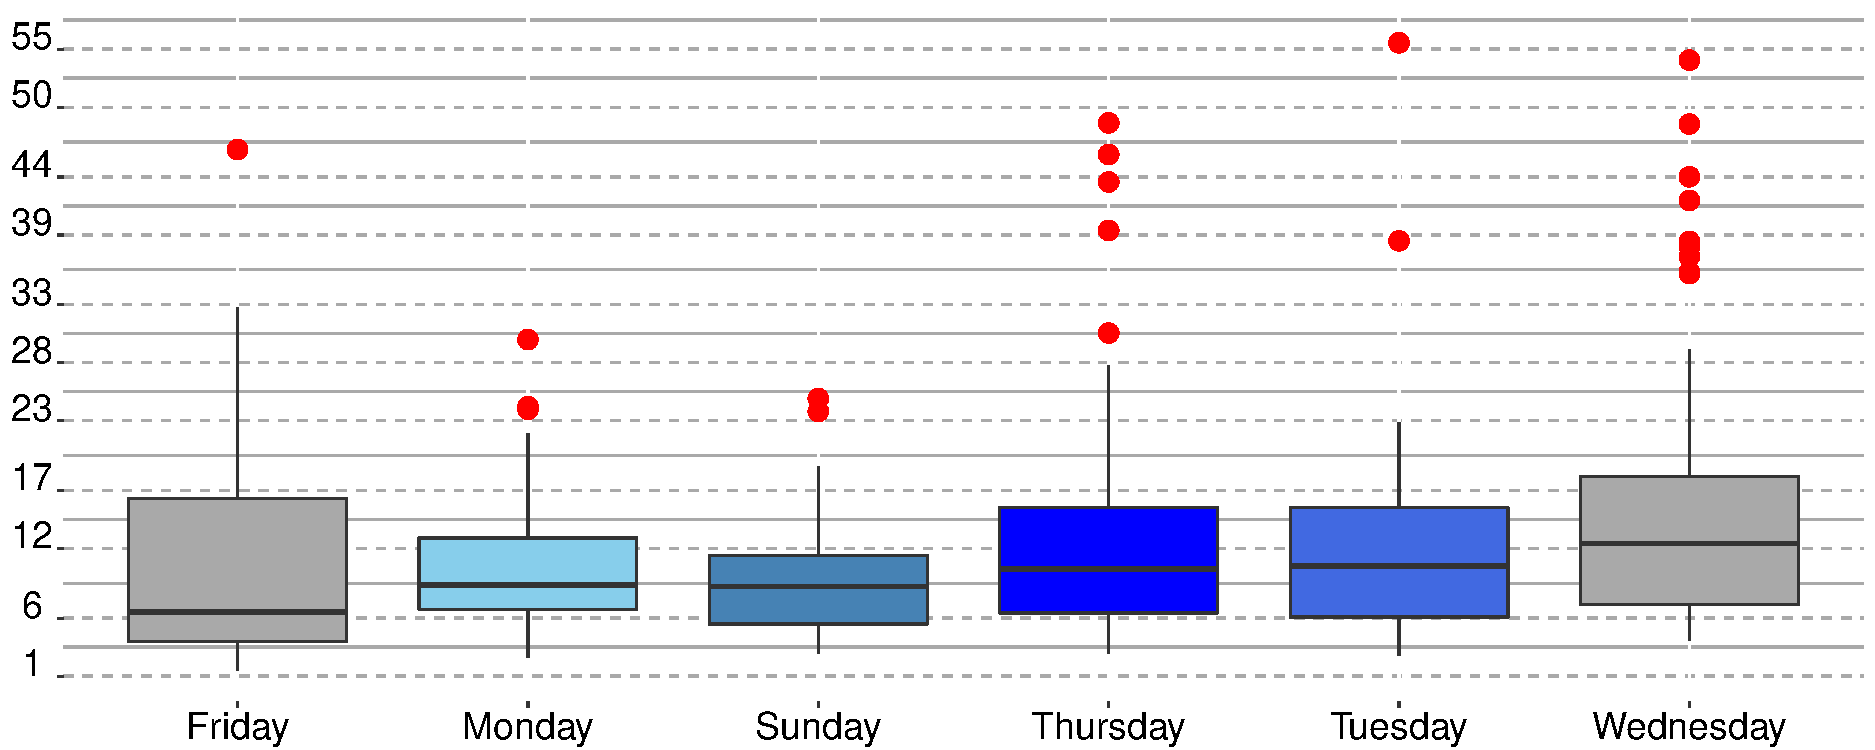
\includegraphics[scale=1]{figure/BP_Plot-2.pdf}
    \end{figure}

  \end{block}
  
\end{column}

\end{columns}

% -- ----------------------------------------------------------------------------------------- -- %
% -- -- Row 5 --   ---------------------------------------------------------------- -- %
% -- ----------------------------------------------------------------------------------------- -- %

\begin{columns}[t]

% -- ------------------------------------------------------------------------------- Columna 1 -- %
% -- ----------------------------------------------------------------------------------------- -- %


\begin{column}{.48 \linewidth}

  \begin{block}{Consecutive Down prices by day}

   \begin{figure}[H]
    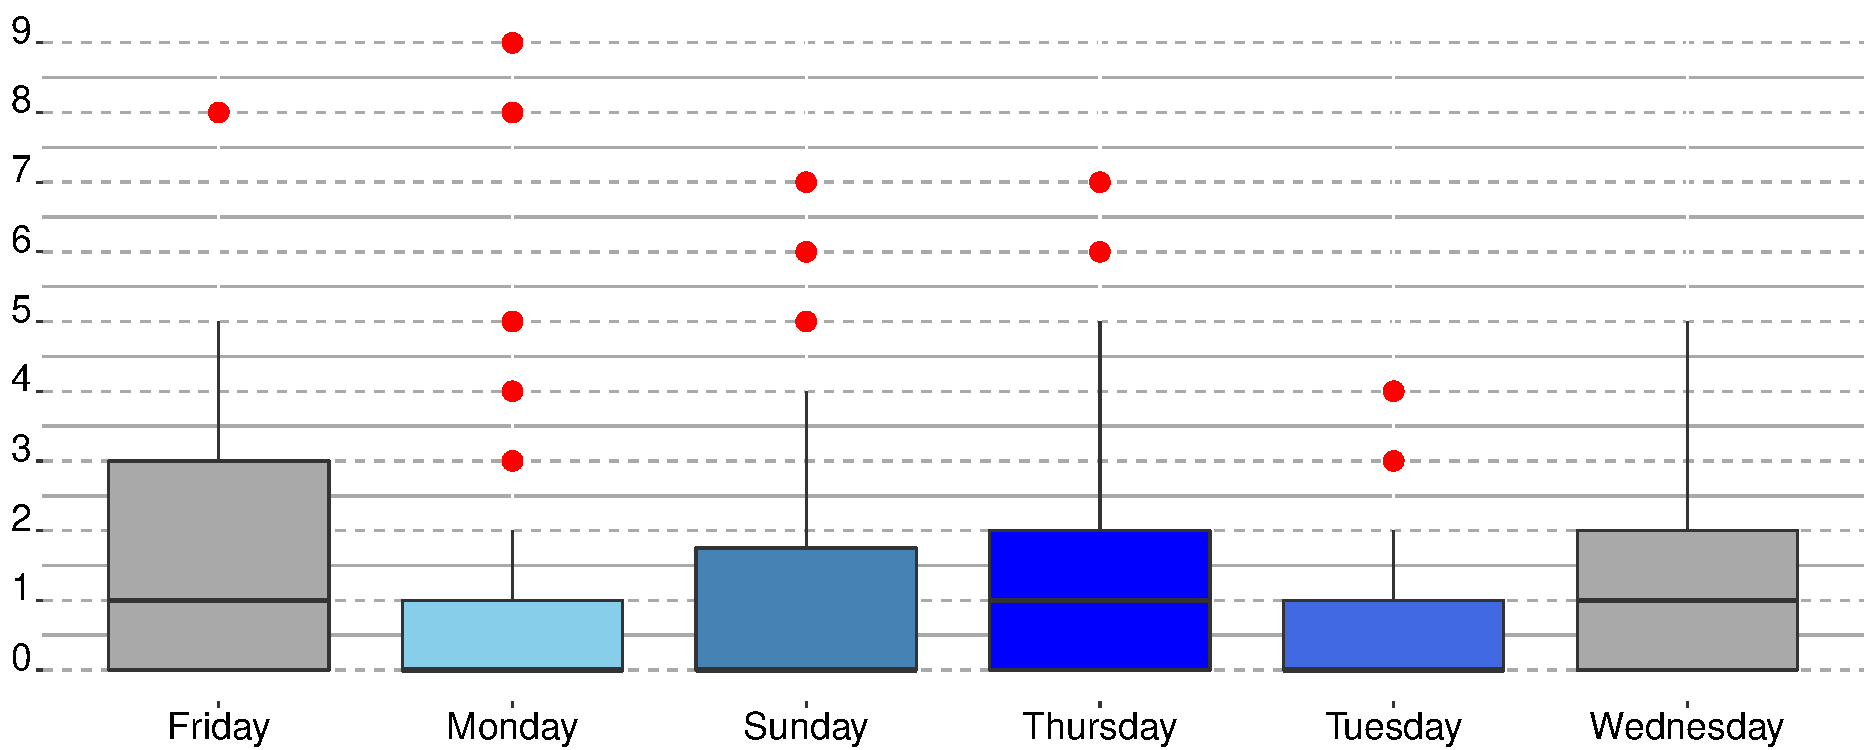
\includegraphics[scale=1]{figure/BP_Plot-3.pdf}
    \end{figure}

  \end{block}
  
\end{column}


% -- ------------------------------------------------------------------------------- Columna 2 -- %
% -- ----------------------------------------------------------------------------------------- -- %

\begin{column}{.48 \linewidth}
  
  \begin{block}{Consecutive Up prices by day}

   \begin{figure}[H]
    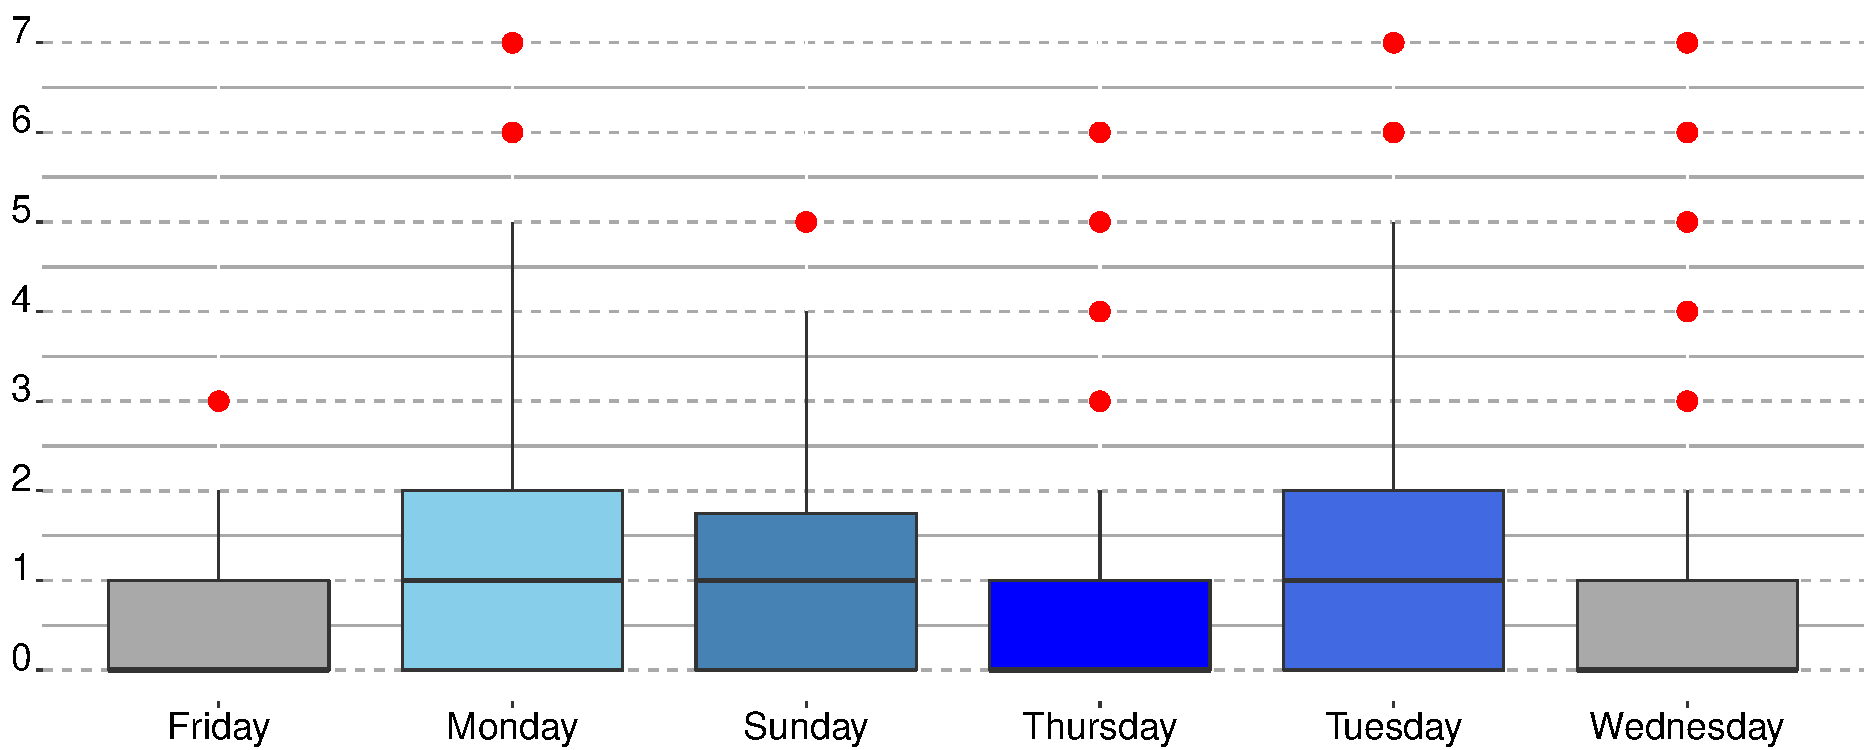
\includegraphics[scale=1]{figure/BP_Plot-4.pdf}
    \end{figure}

  \end{block}
  
\end{column}

\end{columns}


\end{document}
